\section{Federated Learning}
In an era where cloud computing is the dominant paradigm for learning, Federated Learning (FL) has the potential to
drive significant future changes in the industry. Despite the cloud computing market being dominated by
tech giants like Google, Amazon, and Microsoft, Google was the first to recognize the emerging need for a
democratized approach to machine learning. Taking a leading role in Federated Learning research, Google
introduced the term in 2016 with a seminal paper on efficient Distributed Learning\cite{mcmahanCommunicationEfficientLearningDeep2023b}.
The significance of Google’s approach cannot be overstated, as it eliminates the need for maintaining
centralized data centers, allowing cloud resources to be allocated for various other purposes.

% \begin{figure}[!ht]
%     \centering
%     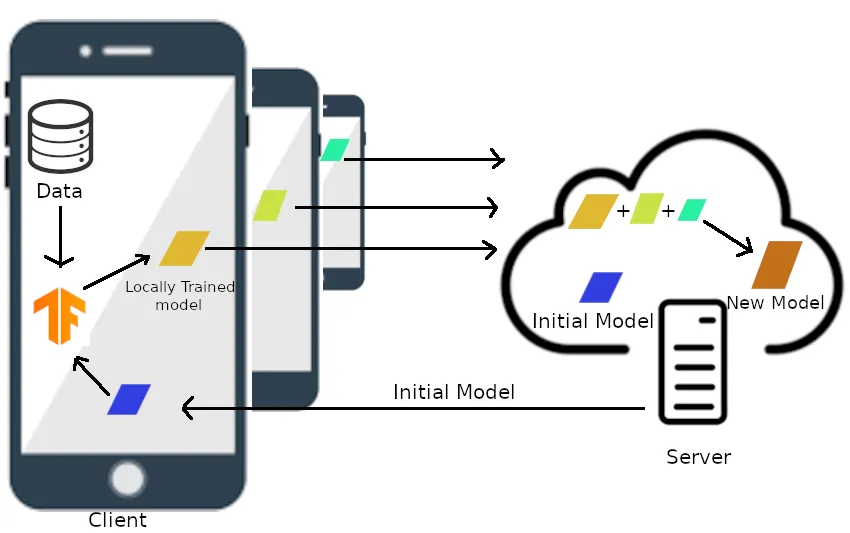
\includegraphics[width=.6\textwidth]{figures/fl/fl.png}
%     \caption{Federated Learning Illustration.}
%     \label{fig:label}
% \end{figure}

The term FL represents a significant shift in how machine learning models are trained and how
data privacy is preserved. As an advanced paradigm within Distributed Machine Learning (DML), FL enables
the training of models across multiple decentralized devices or servers holding local data samples, without
the need to transfer data to a central server. This approach addresses several critical challenges inherent
in traditional centralized machine learning, including data privacy, communication overheads, and the
handling of heterogeneous data and systems.

\begin{figure}[!ht]
    \centering
    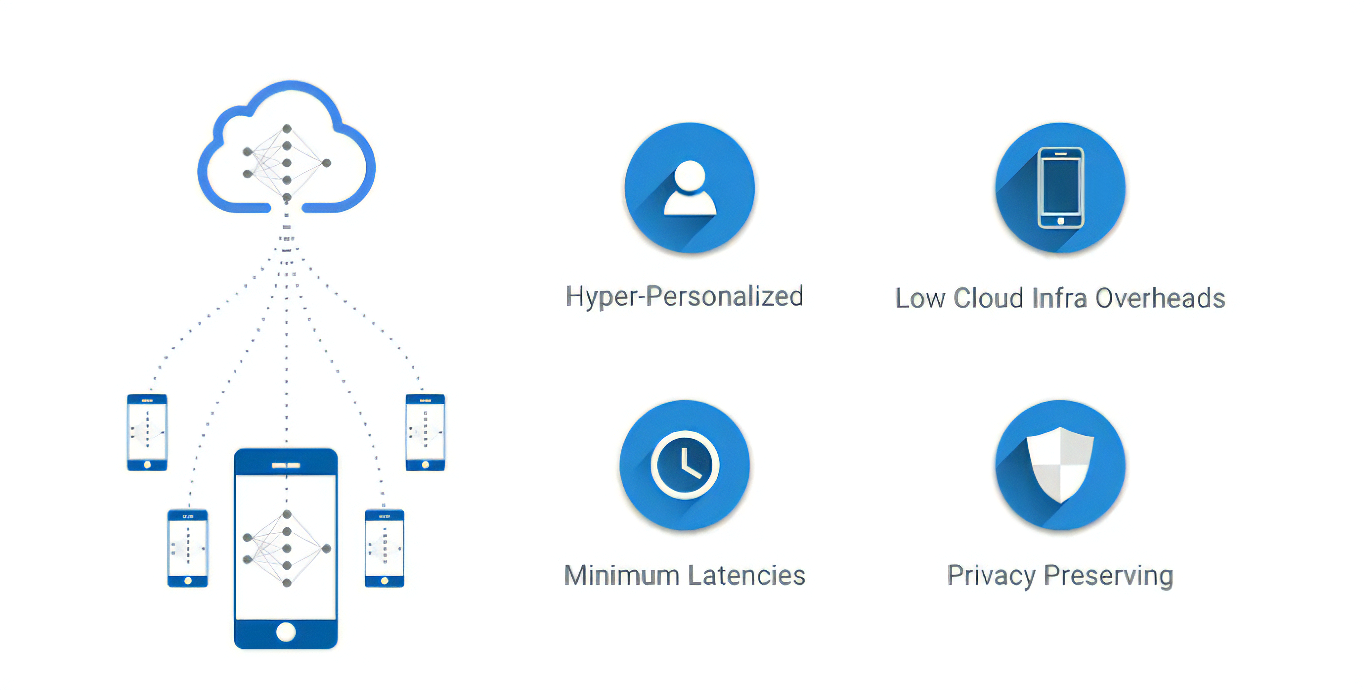
\includegraphics[width=.9\textwidth]{figures/fl/fl_advantages.png}
    \caption{Federated Learning Characteristics.}
    \label{fig:fl_characteristics}
\end{figure}

\subsection{Principles of Federated Learning}
Providing a solution to these issues FL emerged by enabling model training across decentralized devices or
servers while keeping the data local. This method is particularly relevant in scenarios where data privacy is
paramount, such as healthcare, finance, and personal devices like smartphones. A variety of FL applications can
be located in everyday examples-namely image and video automatic categorization, personalized feeds of news
or advertisements, and autocorrect and predictive text (f.i. Google's GBoard\cite{xuFederatedLearningGboard2023}).

\noindent The fundamental principles that determine FL's functionality are categorized as follows\cite{hacksFederatedLearningParadigm2024}:
\begin{itemize}
    \item \emph{Local Data Stays Local:} Data generated by devices or organizations remains on the local device, preventing
          the exposure of sensitive information to external threats or privacy breaches, as it does not need to be uploaded
          to a centralized server for processing.
    \item \emph{Collaborative Model Training:} A central server distributes a global model to devices, which update it based
          on their local data. These updates, typically in the form of gradients or parameters, are sent back to the server and aggregated
          to enhance the global model iteratively, thus improving accuracy and utility without accessing the raw data.
    \item \emph{Privacy by Design:} FL integrates privacy-preserving mechanisms such as secure multi-party computation and
          differential privacy, ensuring that model updates shared with the server do not disclose sensitive information
          about the underlying data or individuals. The privacy rules that are applied, are determined both by international organisms\footnote{Privacy
              preserving legislations such as the General Data Protection Regulation (GDPR) in the European Union
              and the California Consumer Privacy Act (CCPA) in the United States\cite{GeneralDataProtection,CaliforniaConsumerPrivacy}.}
          and local authorities relevant to the region.
    \item \emph{Efficiency and Scalability:} By processing data locally and exchanging only small model updates, FL reduces bandwidth
          requirements for model training, making it scalable across numerous devices and participants, each contributing
          to the refinement of the global model.
\end{itemize}


%%%%%%%%%%%%%%%%%%%%%%%%%%%%%%%%%%%%%%%%%%%%%%%%%%%%%%%%%%%%%%%%%%%%%%%%%%%%%%%%%%%%%%%%%%%%%%%%%%%%%%%%%%%%%%%%%%%%%%%%%%%%%%%%%%%%%%%%%%%%%%%%%%%%%%%%%%%%%%
\subsection{Federated Learning Categorizations}
Several criteria can be used to determine a holistic categorization of Federated Learning (FL) approaches\cite{caruccioSurveyingFederatedLearning2024}.
For the purpose of this research study, the two principal factors are the scale of learning and the alignment of the distributed data. Based on
the learning scale, the separation is executed into Cross-Device and Cross-Silo settings. Based on the data distribution, the
categorization is between Horizontal and Vertical learning settings. The terms presented above will be explained next:

\paragraph{Nature of the Participants:} The distinction is based on whether the federated learning system involves numerous personal
or edge devices (cross-device) or a smaller number of institutions or organizations (cross-silo).

\paragraph{Alignment of the Distributed Data:} The distinction is based on whether the datasets across entities share the same feature
space but have different samples (horizontal) or share the same sample space but have different features (vertical).

%%%%%%%%%%%%%%%%%%%%%%%%%%%%%%%%%%%%%%%%%%%%%%%%%%%%%%%%%%%%%%%%%%%%%%%%%%%%%%%

\begin{figure}[!ht]
    \centering
    \begin{subfigure}[b]{0.45\textwidth}
        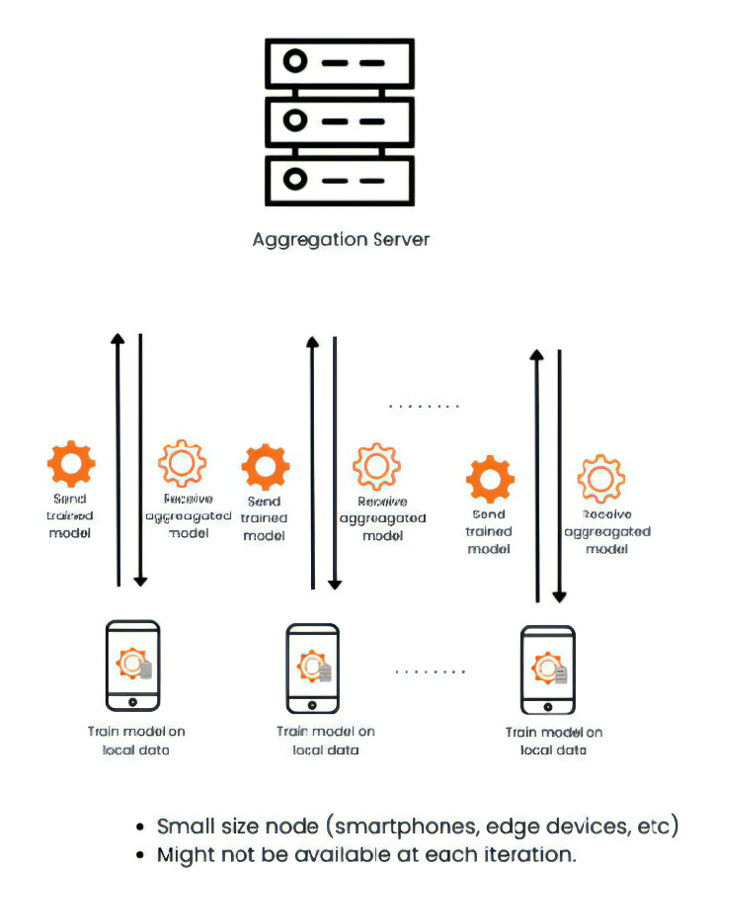
\includegraphics[width=\textwidth]{figures/fl/devices.png}
        \caption{Cross-Device Learning.}
        \label{fig:device}
    \end{subfigure}
    \hfill
    \begin{subfigure}[b]{0.45\textwidth}
        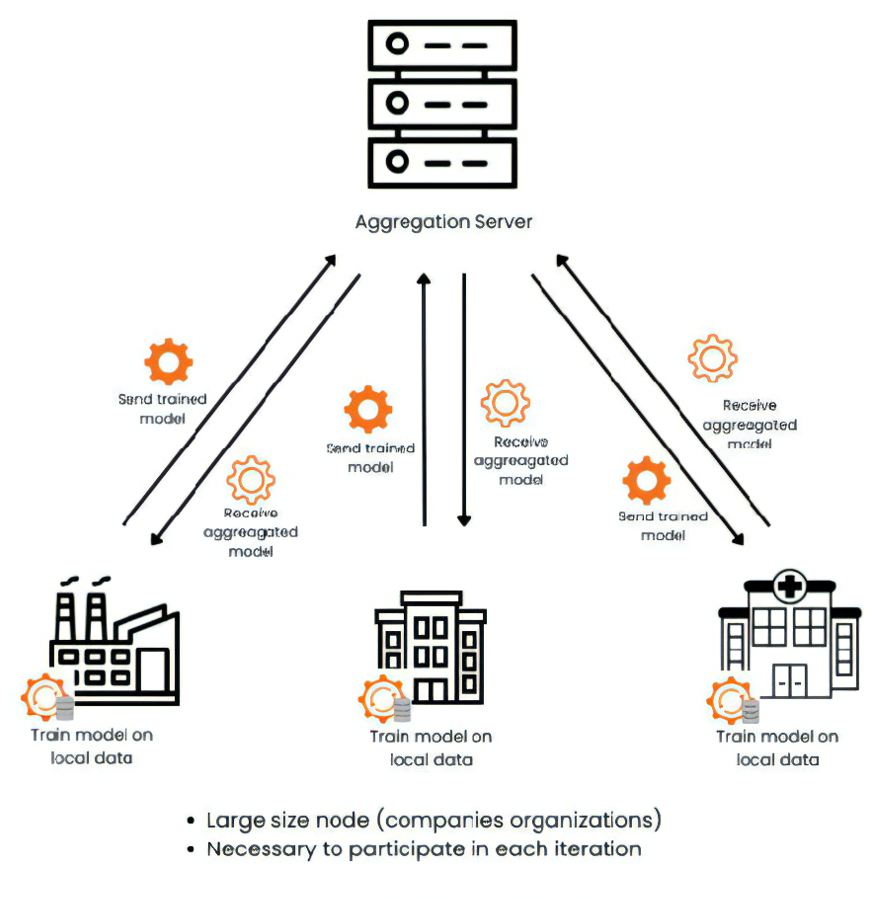
\includegraphics[width=\textwidth, height=1.15\textwidth]{figures/fl/silos.png}
        \caption{Cross-Silo Learning.}
        \label{fig:silo}
    \end{subfigure}
    \caption{Federated Systems separation in Cross-Device or Cross-Silo scale}
    \label{fig:fl_cat_scale}
\end{figure}

\paragraph{Cross-Device Federated Learning}
Cross-device FL involves training models on a large number of edge devices such as smartphones and IoT devices (see \cref{fig:device}). Each device
holds a small, local dataset. This type of FL is particularly useful for applications where individual user data is sensitive,
and thus cannot be shared directly. The primary challenges include managing the diversity in device capabilities, ensuring
efficient communication, and maintaining data privacy. Techniques like asynchronous updates and efficient gradient compression
are often employed to address these challenges\cite{mcmahanCommunicationEfficientLearningDeep2023,chenDistributedLearningWireless2021}
%%%%%%%%%%%%%%%%%%%%%%%%%%%%%%%%%%%%%%%%%%%%%%%%%%%%%%%%%%%%%%%%%%%%%%%%%%%%%%%
\paragraph{Cross-Silo Federated Learning}
Cross-silo FL is used when a small number of organizations, such as hospitals or financial institutions, collaborate to
train a machine learning model (see \cref{fig:silo}). Each organization (silo) has a larger dataset, but data cannot be shared due to privacy concerns.
This method often aligns with regulatory requirements such as GDPR and CCPA\@. Challenges include managing non-IID data distributions
across silos and ensuring secure aggregation of model updates. Techniques like secure multi-party computation (SMPC) and differential
privacy are crucial in this context\cite{yangFederatedMachineLearning2019,zhaoFederatedLearningNonIID2018}.


%%%%%%%%%%%%%%%%%%%%%%%%%%%%%%%%%%%%%%%%%%%%%%%%%%%%%%%%%%%%%%%%%%%%%%%%%%%%%%%
%%%%%%%%%%%%%%%%%%%%%%%%%%%%%%%%%%%%%%%%%%%%%%%%%%%%%%%%%%%%%%%%%%%%%%%%%%%%%%%%%%%%%%%%%%%%%%%%%%%%%%%%%%%%%%%%%%%%%%%%%%%%%%%%%%%%%%%%%%%%%%%%%%%%%%%%%%%%%%
\subsubsection{Horizontal and Vertical Federated Learning}

\paragraph{Horizontal Federated Learning (HFL)}
HFL, or sample-based FL, occurs when different entities (devices or institutions) have datasets with the same feature space
but different samples. For instance, multiple hospitals might have patient records with the same attributes. HFL is commonly
used in both cross-device and cross-silo settings. The main challenge is handling non-IID data, where each client’s data
distribution may vary significantly. Approaches like data augmentation and federated averaging (FedAvg) are often used to
mitigate these issues\cite{konecnyFederatedOptimizationDistributed2016}.

%%%%%%%%%%%%%%%%%%%%%%%%%%%%%%%%%%%%%%%%%%%%%%%%%%%%%%%%%%%%%%%%%%%%%%%%%%%%%%%
\paragraph{Vertical Federated Learning (VFL)}
VFL, or feature-based FL, occurs when entities have datasets with different feature spaces but the same sample space. For
example, one organization might have transaction data, while another has demographic data about the same customers. VFL is
typically used in cross-silo settings. The primary challenge is ensuring secure and efficient computation when combining
different types of data. Secure computation techniques and feature alignment methods are critical to address these challenges
~\cite{yangFederatedMachineLearning2019,chenDistributedLearningWireless2021}.

\begin{figure}[!ht]
    \centering
    \begin{subfigure}[b]{0.45\textwidth}
        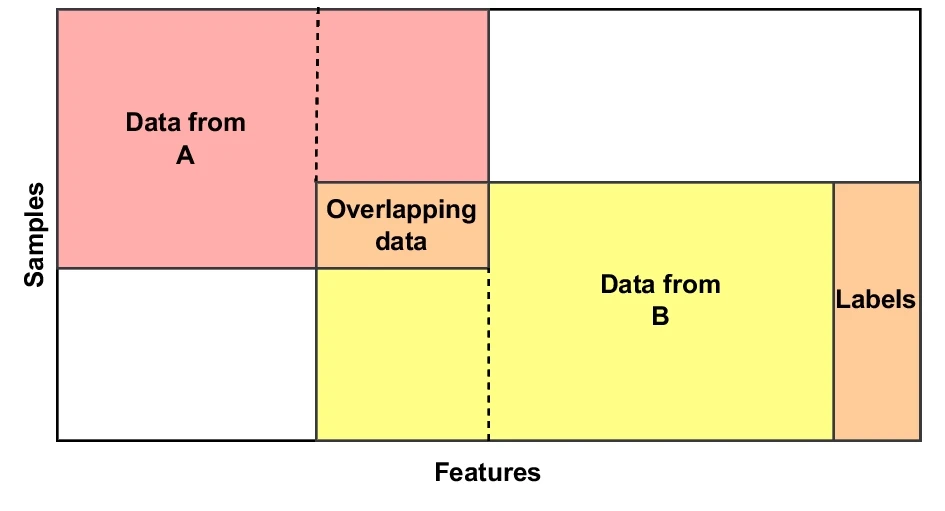
\includegraphics[width=\textwidth]{figures/fl/horizontal.png}
        \caption{Horizontal Federated Learning.}
        \label{fig:horizontal}
    \end{subfigure}
    \hfill
    \begin{subfigure}[b]{0.45\textwidth}
        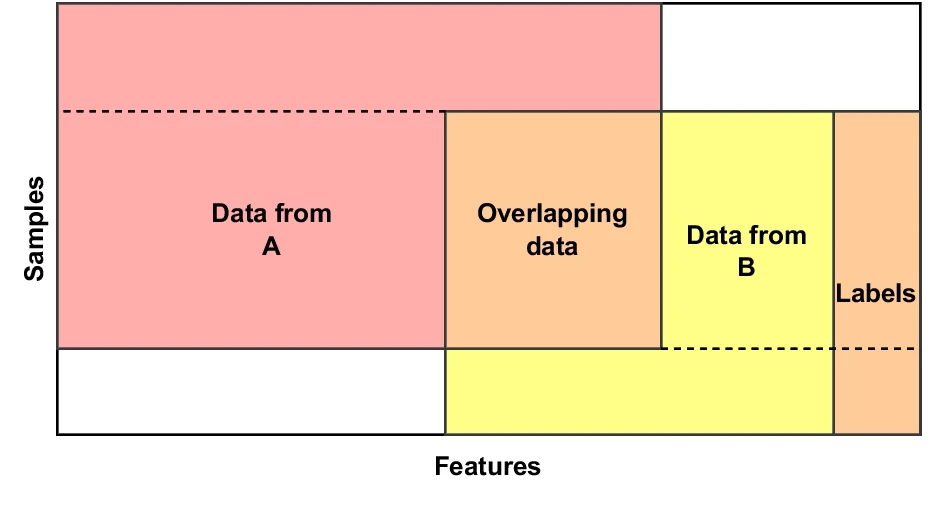
\includegraphics[width=\textwidth]{figures/fl/vertical.png}
        \caption{Vertical Federated Learning.}
        \label{fig:vertical}
    \end{subfigure}
    \caption{Federated Systems separation in horizontal or vertical learning\cite{caruccioSurveyingFederatedLearning2024}.}
    \label{fig:fl_cat_distribution}
\end{figure}
%%%%%%%%%%%%%%%%%%%%%%%%%%%%%%%%%%%%%%%%%%%%%%%%%%%%%%%%%%%%%%%%%%%%%%%%%%%%%%%
%%%%%%%%%%%%%%%%%%%%%%%%%%%%%%%%%%%%%%%%%%%%%%%%%%%%%%%%%%%%%%%%%%%%%%%%%%%%%%%%%%%%%%%%%%%%%%%%%%%%%%%%%%%%%%%%%%%%%%%%%%%%%%%%%%%%%%%%%%%%%%%%%%%%%%%%%%%%%%
\subsection{Federated Learning Methodology}
\subsubsection{Architecture}
In a Federated Learning setup, the architecture can be decomposed into four principal parts:
The client devices, the central server, the communication protocols, and the security mechanisms.
An overview of each component's functionality will be presented for a typical Federated Learning Architecture
based on the cumulative analysis provided by multiple
literature sources\cite{mcmahanCommunicationEfficientLearningDeep2023,yangFederatedMachineLearning2019,
    konecnyFederatedOptimizationDistributed2016,bhoseDifferentiatingDistributedLearning2023}.
It is avoided to delve further into details for some of the presented terms in cases where they are not
relevant to the research's objectives. In those circumstances, just a conceptual illustration is provided.

\paragraph{Client Devices:} Client devices are the edge devices or local servers that generate and hold the local data.
These can include smartphones, IoT devices, or organizational databases. Each client device performs local training on
its dataset, updating the model’s parameters based on local data. This helps preserve data privacy since the raw data
never leaves the device. After training locally, the clients send their model updates (e.g., gradients or parameters)
to the central server. These updates are computed using the local data, ensuring that sensitive or personal information
is not exposed. The heterogeneity of these devices, in terms of computational power and network connectivity, presents
a challenge that must be managed by the system.

\paragraph{Central Server:} The central server acts as a coordinator that aggregates model updates from multiple
client devices and updates the global model. Essentially, the server collects model updates sent by the clients, aggregates
these updates to refine the global model, and then redistributes the updated global model back to the clients for further
training iterations. This process ensures that the global model improves iteratively based on the decentralized data from
all participating clients. The central server must handle the challenges of aggregating updates efficiently and securely
to maintain the model's performance and integrity.

\paragraph{Communication Protocols:}\label{par:communication} The communication protocol defines the rules and methods for data exchange between
client devices and the central server. Efficient communication protocols are essential to minimize latency and bandwidth
usage during the model update exchanges. Protocols in FL often incorporate techniques to reduce the volume of data transferred,
such as model compression and gradient sparsification. Asynchronous communication methods can handle the varying availability and
performance of client devices, reducing overall training time and mitigating the straggler effect.

\paragraph{Security Mechanisms:}\label{par:security} Security mechanisms are critical in FL to ensure that the data and model updates remain confidential and tamper-proof.
These mechanisms protect against potential attacks that could compromise the privacy and integrity of the data being processed.
Common security measures include encryption, differential privacy, and secure multi-party computation (SMPC). Encryption ensures that data
transmitted between clients and the server is protected from eavesdropping. Differential privacy adds noise to the model updates to prevent the
reconstruction of sensitive data. SMPC allows multiple parties to compute a function over their inputs while keeping those inputs private, further
enhancing the security of the federated learning process.

%%%%%%%%%%%%%%%%%%%%%%%%%%%%%%%%%%%%%%%%%%%%%%%%%%%%%%%%%%%%%%%%%%%%%%%%%%%%%%%%%%%%%%%%%%%%%%%%%%%%%%%%%%%%%%%%%%%%%%%%%%%%%%%%%%%%%%%%%%%%%%%%%%%%%%%%%%%%%%
\subsection{Problem Formulation in Federated Learning}
This section provides a clear a clear overview of the FL problem statement based on the Almanifi et al.\ article (2023)\cite{almanifiCommunicationComputationEfficiency2023}
observations.
In the broader field of Machine Learning (ML), the primary problem is to learn a model that maps a set of input data \( x \) to a set of
desired outputs \( y \) based on a number of training examples. The performance of this model is evaluated using a loss function \( f_i(w) \),
which measures the error between the model's predictions and the actual desired outputs. For a set of \( n \) input-output pairs $\{x_i, y_i\}_{i=1}^n$,
the goal is to find the optimal weight vector(s) \( w \) that minimizes the loss function. An example of this in a linear regression problem is:

\begin{equation}
    f_i(w) = \frac{1}{2}(x_i^T w - y_i)^2, \quad y_i \in \mathbb{R} \text{ and } x_i \in \mathbb{R}^d
\end{equation}

Although loss functions vary across different ML techniques, the problem generally can be formulated as an optimization problem for a
finite-sum of functions, expressed as:

\begin{equation}
    \label{eq:objctive_func_fedAVG}
    \min_{w \in \mathbb{R}^d} f(w) \quad \text{where} \quad f(w) = \frac{1}{n} \sum_{i=1}^n f_i(w)
\end{equation}

In Federated Learning, the training process minimizes the loss function locally through gradient descent before the
weights \( w \) are communicated to the central server. Consider an FL system
with a fixed number of clients \( K \), where each client hosts a partition of the data \( n_k \), indexed by
\( \mathcal{P}_k = \{1, 2, \ldots, i\} \). Upon receiving all local parameters, the global server aggregates \( w \) to update the
new global model. The aggregation mechanism sets the global objective. For example, in FedAVG, one of the most commonly used aggregation
methods in FL, the loss function is updated to:

\begin{equation}
    f(w) = \sum_{k=1}^K \frac{n_k}{n} F_k(w) \quad \text{where} \quad F_k(w) = \frac{1}{n_k} \sum_{i \in \mathcal{P}_k} f_i(w)
\end{equation}

Thus, the problem in FL becomes learning the aforementioned model in a distributed manner without exchanging raw data.

%%%%%%%%%%%%%%%%%%%%%%%%%%%%%%%%%%%%%%%%%%%%%%%%%%%%%%%%%%%%%%%%%%%%%%%%%%%%%%%%%%%%%%%%%%%%%%%%%%%%%%%%%%%%%%%%%%%%%%%%%%%%%%%%%%%%%%%%%%%%%%%%%%%%%%%%%%%%%%
\subsubsection{Federated Learning Process} \label{sec:fed_learning_process}
\begin{figure}[!ht]
    \centering
    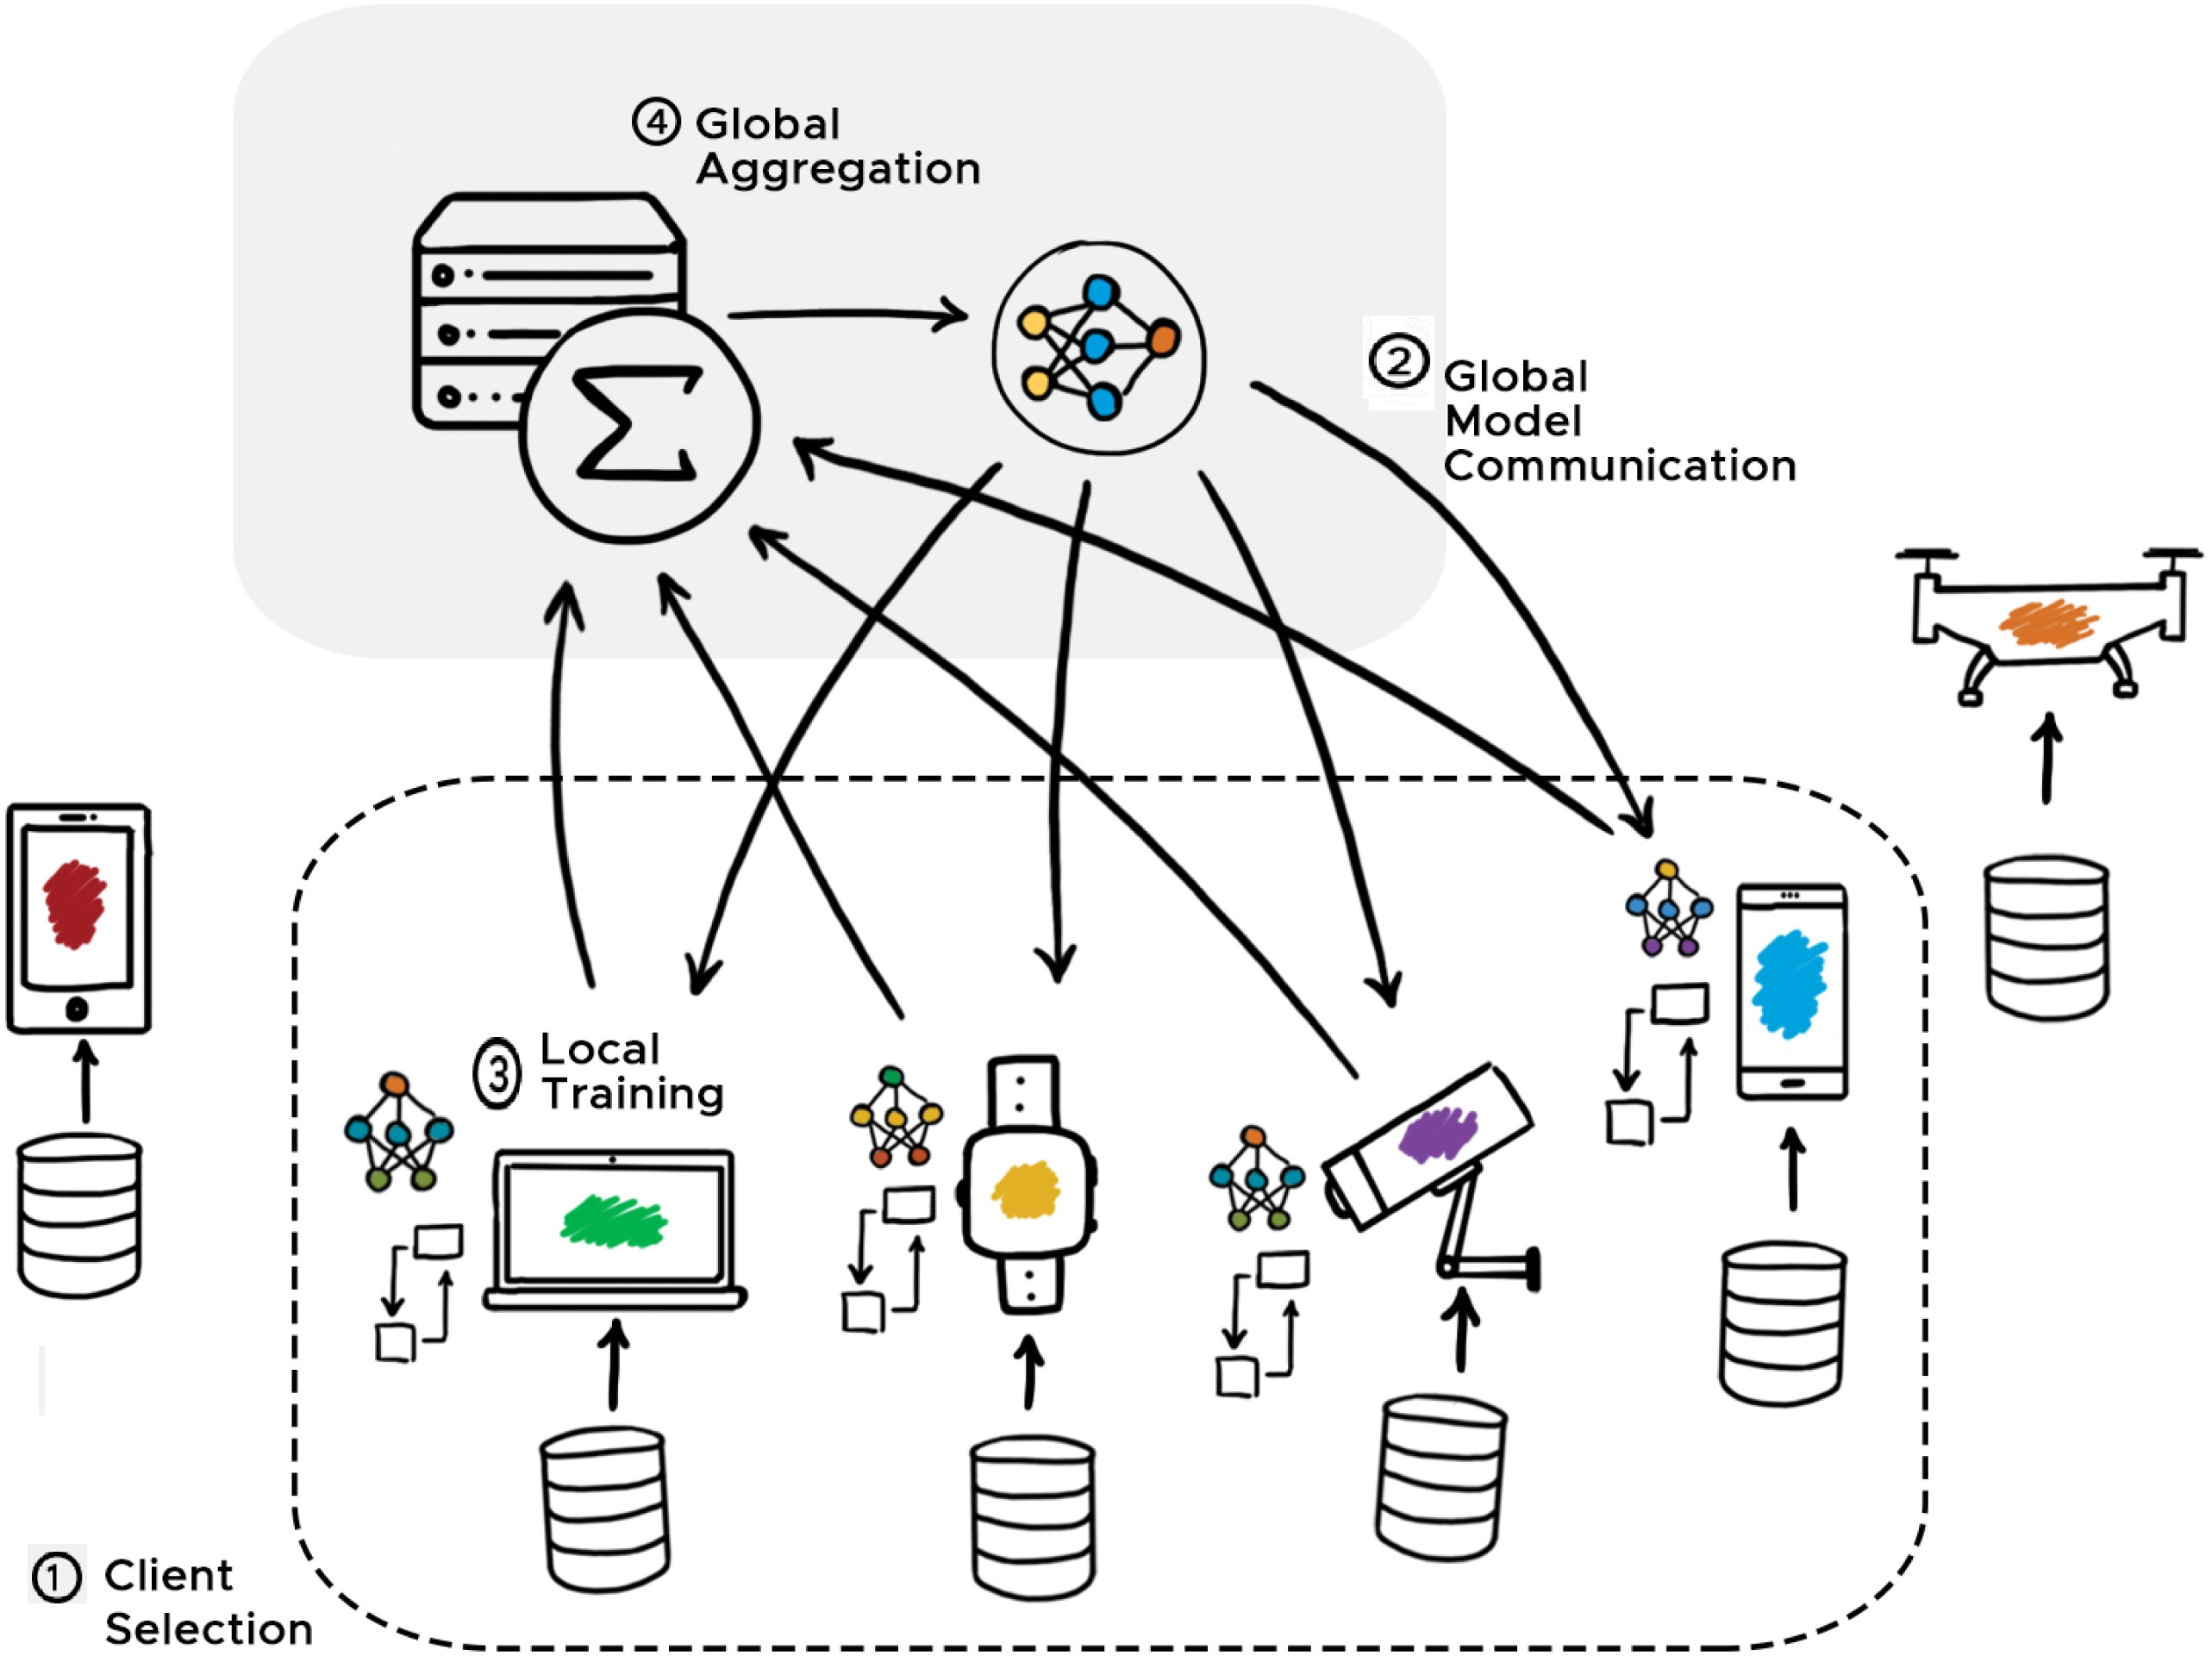
\includegraphics[width=.8\textwidth]{figures/fl/fl_2.jpg}
    \caption{General FL training process\cite{almanifiCommunicationComputationEfficiency2023}.}
    \label{fig:fl_process}
\end{figure}

In distributed machine learning setups, such as Federated Learning, processes are often viewed as continuous, meaning that the system continuously
updates and refines the model parameters based on incoming data. This continuous process allows for dynamic adjustments and real-time improvements,
making the system more adaptive and responsive to changes in the data\cite{deanLargeScaleDistributed2012,almanifiCommunicationComputationEfficiency2023}.
Provided that, in the iterative training process, each iteration/round can be separated into four major steps as displayed in \cref{fig:fl_process}:

\begin{enumerate}

    \item \emph{Client Selection:} Selection strategies vary, as client selection can be executed either randomly, or with prioritization criteria in mind.
          Depending the FL setup, client selection can be conducted at two different stages: either before sending the global model
          to the clients (first step) or after local training (third step).
          \emph{First Step Selection}: The central manager selects a subset of clients before sending the global model. This pre-selection
          can be used to restrict the number of clients that participate in training, while also gives the opportunity to filter clients based
          on their update quality.
          \emph{Third Step Selection}: After local training, the server selects a subset of clients to transmit their model updates. This step
          prevents diminishing returns seen when the full set of clients is used.  In our implementation client selection is conducted before the
          global model communication.

    \item \emph{Global Model Communication:} The process begins with available clients notifying the server of their readiness to participate. The server then
          communicates the global model to all participating clients, signaling the beginning of the communication round. This step involves broadcasting the global
          model's parameters, which include weights and biases, along with any relevant metadata such as hyperparameters (e.g., learning rate) and other arguments
          (e.g., batch size).

    \item \emph{Local Training:} Each client trains the model locally using its own local dataset. During this step, the clients adjust the global model
          parameters based on their local data, resulting in a \emph{Model Update}. The training process is conducted according to the instructions and
          hyperparameters provided by the server. The objective function of the training process is notated as \( f \), and for a selected client \( n \)
          from the set of clients \( N \), it attempts to minimize its loss function \( L \), which depends on the global model weights \( w_g \) and the
          local data \( d_i \):

          \begin{equation}
              f_n(w_g) = \arg\min_{n \in N} L(w_g; d_n)
          \end{equation}
          After training, clients need to transmit their model updates back to the central server for aggregation (see \cref{en:aggregation}).
          The model updates may undergo additional processing to enhance efficiency and security, as outlined in \cref{par:communication}.
          Finally, the processed model updates are transmitted to the server, and the clients remain inactive until selected again.

    \item \emph{Global Aggregation:}\label{en:aggregation}
          Upon receiving the updated parameters from each selected client, the server aggregates them into a global model using a chosen aggregation
          mechanism. Various strategies can be employed, such as the FedAVG method, which averages the updates from the clients. The global objective
          is to minimize the overall loss function as shown in \cref{eq:objctive_func_fedAVG}. Once the model is updated, the communication round ends.
          The server then evaluates the global model's performance using metrics over a public test set. Based on this evaluation, training may be
          terminated if the desired accuracy is achieved or the preset number of rounds is completed; otherwise, a new communication round begins.
\end{enumerate}

The above functionality describes a synchronous federated learning setup, which aligns with the thesis implementation. However, as highlighted earlier
in order to improve a distributed system's performance, asynchronous methods can be applied too, mitigating the straggler effect.

% While programming an asynchronous learning system is taxing and requires careful considerations about out-of-sync updates, the fundamental logic remains the same.
% Building on the outlined learning procedure above, the only things that would be modified in a asynchronous setup, is the removal of synchronization 
% mechanisms. Specifically, unlike the synchronous counterpart, in asynchronous clients can start and finish training in different times. 

While programming an asynchronous learning system is taxing and requires careful considerations about out-of-sync updates, the fundamental logic remains the same
with modifications primarily pertain to the timing and coordination of these steps. To be exact, In an asynchronous federated learning setup, client selection remains dynamic,
but clients are allowed to start and finish their local training at different times. This flexibility means that the server can receive and aggregate updates from
clients as they become available, without waiting for all selected clients to complete their training. Consequently, global model communication is also more fluid,
with the server sending the global model to clients on an as-needed basis, rather than all at once. Local training on each client still follows the same process,
but clients send their updates to the server independently upon completion. The server continuously aggregates these updates using the chosen aggregation mechanism,
such as weighted averaging, and updates the global model iteratively.

